\section{Identificação de Sistemas Instáveis}

A identificação de sistemas é a área voltada à obtenção de modelos a partir de dados experimentais de entrada e saída, conforme apresenta a Figura \ref{identification-model}, em contraposição à modelagem caixa branca, derivada unicamente das leis físicas do processo. Existem dois tipos de identificação de sistemas, o método de caixa preta, onde o modelo é obtido exclusivamente a partir dos dados, e de caixa cinza, que combina uma estrutura física conhecida com a estimação de parâmetros baseada em medições \cite{Aguirre2015}. 

Este trabalho enquadra-se na abordagem de caixa cinza, pois parte da estrutura física do modelo de corpo rígido, deduzida no Capítulo~2, e estima seus parâmetros a partir de dados reais de voo.

\begin{figure}[ht]
    \centering
    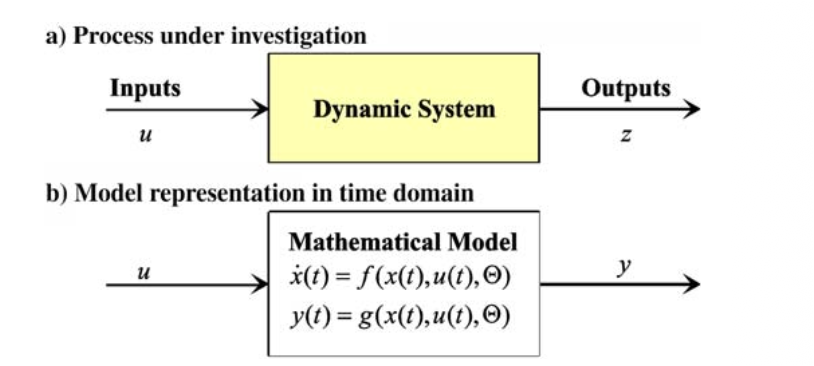
\includegraphics[width=0.7\textwidth]{Cap3/identification2.png}
    \caption{Modelagem Matemática de um Sistema Físico \cite{Jategaonkar2015}.}
    \label{identification-model}
\end{figure}

O processo de identificação compara, a partir de um mesmo sinal de entrada $u$, a medição do sistema dinâmico e a saída do modelo matemático, para estimação dos melhores parâmetros e estruturas para representar esse processo físico \cite{Aguirre2015}. Porém, como apresentado em \textcite{Jategaonkar2015}, determinados tipos de sistemas são instáveis a entrada em malha aberta, portanto, necessitam de um controlador para que seja possível observar o sistema e realizar a identificação.

Considerando a Figura \ref{identification-diagram} para identificar o sistema $\mathbf{H}$, com o sinal de entrada $u$ e a medição dos sensores $z$, existem duas abordagens diferentes, onde a primeira observa o conjunto completo indicada como identificação por malha-fechada, relacionando as entradas de comando $\boldsymbol{\sigma_P}$ com a saída $z$, a qual é recomendada para processos em que se deseja apenas reproduzir o comportamento global, de comando para resposta. Por reunir a planta e o controlador em um único modelo equivalente, o sistema observado permanece estável, de forma que qualquer método padrão de estimação, como o método do erro de saída, pode ser aplicado sem dificuldades numéricas. Sua principal limitação, contudo, é fornecer apenas esse modelo equivalente do conjunto, sem separar os parâmetros da aeronave da dinâmica do controlador \cite{Jategaonkar2015}.

A segunda abordagem é a identificação em malha aberta dentro do sistema controlado, o qual visa caracterizar diretamente a planta $\mathbf{H}$, o VTOL instável isolado, relacionando a entrada efetiva $u$, aplicada pelo controlador, com a saída medida $z$, como utilizado nos trabalhos de \textcite{Matt2025, Niermeyer2015}. É esta a abordagem adotada neste trabalho, por permitir estimar os parâmetros físicos do próprio drone, e não um modelo equivalente do conjunto planta-controlador. Em contrapartida, a integração de um sistema inerentemente instável pode conduzir à divergência numérica, ou correlação forte entre entrada e saída, quando é empregado o método do erro de saída clássico, exigindo cuidados específicos no processo de estimação \cite{Jategaonkar2015,Tischler2012}.

\begin{figure}[ht]
    \centering
    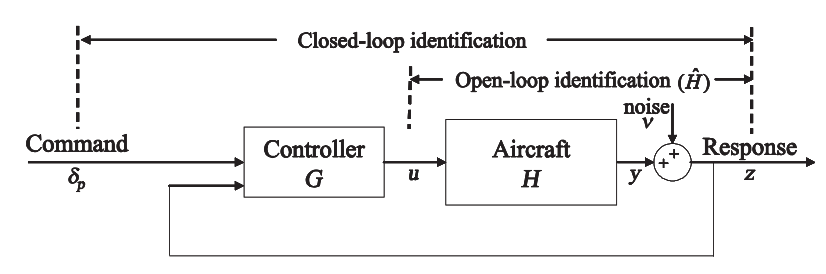
\includegraphics[width=0.8\textwidth]{Cap3/identification.png}
    \caption{Identificação de Sistemas Instáveis com Controlador \cite{Jategaonkar2015}.}
    \label{identification-diagram}
\end{figure}

\section{Método de Identificação M4V}

A metodologia de identificação sugerida por \textcite{Jategaonkar2015} é o M4V, uma abordagem sistemática e iterativa para a identificação de sistemas dinâmicos no domínio do tempo, muito utilizada na identificação de aeronaves \cite{Jategaonkar2015, Tischler2012}. O objetivo é obter uma identificação confiável, através do processamento das medições de forma adequada, utilizando métodos de otimização e modelos matemáticos representativos, de forma que os parâmetros obtidos realmente sejam úteis para simulação e projeto de controle.  A sigla reúne as cinco etapas que estruturam o processo, os quatro \textit{M}, das iniciais dos termos em inglês, e o \textit{V} de validação, executadas de forma iterativa, até que o modelo atenda aos critérios de validação estabelecidos, conforme detalhado no diagrama da Figura \ref{m4v}. 

\begin{figure}[ht]
    \centering
    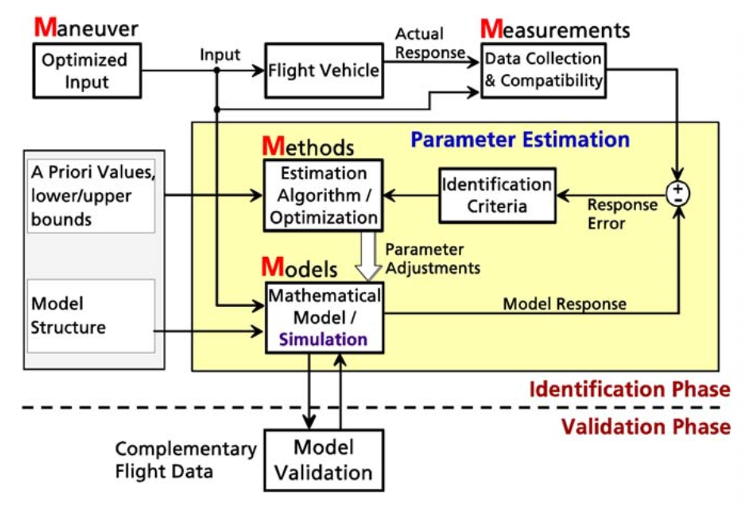
\includegraphics[width=0.8\textwidth]{Cap3/m4v.png}
    \caption{Diagrama da metodologia de identificação M4V \cite{Jategaonkar2015}.}
    \label{m4v}
\end{figure}

Essas etapas, detalhadas nas subseções a seguir, são:

\begin{itemize}
    \item \textbf{Manobras} (\textit{Maneuvers});
    \item \textbf{Medições} (\textit{Measurements});
    \item \textbf{Métodos} (\textit{Methods});
    \item \textbf{Modelos} (\textit{Models});
    \item \textbf{Validação} (\textit{Validation}).
\end{itemize}

\subsection{Definição de manobras (Maneuvers)}

Diferentemente das aeronaves de asa fixa, que podem ser excitadas em torno de uma condição de voo trimada e naturalmente estável, o quadrirrotor é instável e opera em malha fechada, estabilizado por um controlador em torno do voo pairado. A excitação não é aplicada diretamente à planta, mas injetada como uma entrada exógena, somada à saída do controlador.  Portanto, \textcite{Jategaonkar2015} sugere que as manobras sejam aplicadas um eixo de cada vez, procedimento denominado \textit{separate surface excitation} a qual reduz significantemente a correlação que a realimentação impõe entre entrada e estados, vale ressaltar que este procedimento é determinado para um modelo de asa-fixa, mas utilizado como base teórica para definição de manobras com o multirrotor controlado. Para que a dinâmica de cada eixo seja isolada e identificável, a excitação precisa ser suficientemente diferenciada do equilíbrio, pois, se a entrada for pequena, o controlador suprime o transitório e mascara a planta \cite{Jategaonkar2015}.

Cabe ressaltar que, em voo pairado, cada taxa angular obedece a uma dinâmica de primeira ordem, enquanto atitude e velocidade formam uma cadeia de integradores acoplados pela gravidade, origem da instabilidade que torna a malha fechada necessária. Por isso, a frequência $\omega_n$ empregada no dimensionamento da manobra deve ser entendida como a frequência característica do canal que se deseja identificar, onde a banda da dinâmica de taxa é governada por $c_p,c_q,c_r$ e pela efetividade de controle, e não como um período curto aerodinâmico.

Distinguem-se, dessa forma, três sinais ao longo da cadeia de excitação: O comando do piloto $\boldsymbol{\sigma_P}$ (canais de rádio) que é a entrada exógena de referência, depois tem-se o controlador que soma esse comando junto com a ação de estabilização, e através da inversa da matriz de alocação, apresentada em \eqref{eq:alocacao} $\mathbf{B^{-1}}$, também chamado de mixer, atribui um valor de PWM aos quatro motores ($\sigma_1, \sigma_2, \sigma_3, \sigma_4$). Desses comandos PWM obtêm-se, pela mesma alocação adotada no estimador, os momentos generalizados que efetivamente atuam sobre o corpo, conforme apresenta a Figura \ref{cadeia}:

\begin{figure}[ht]
    \centering
    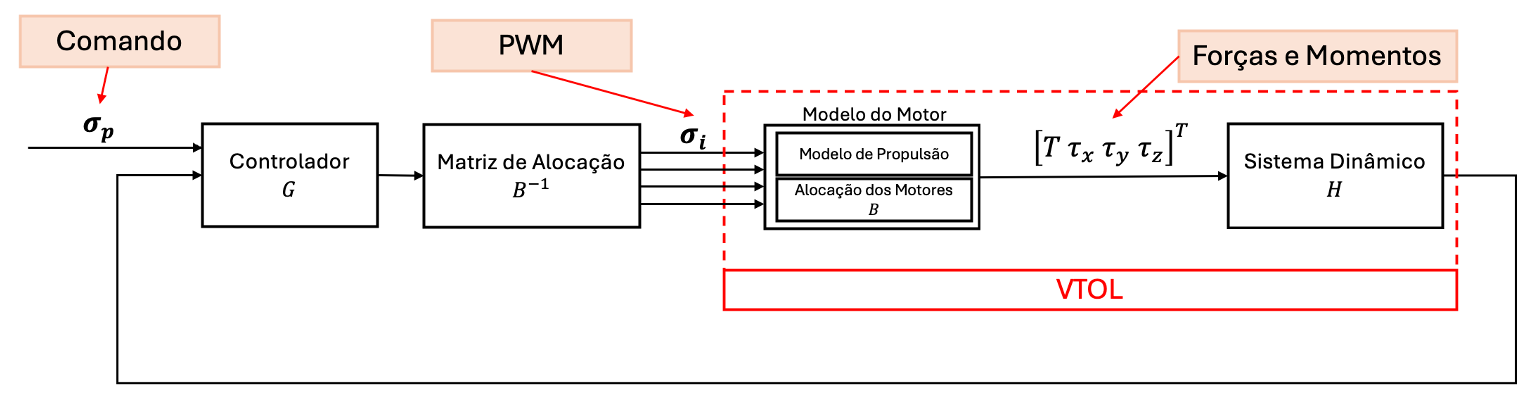
\includegraphics[width=1\textwidth]{Cap3/entradas.png}
    \caption{Cadeia de excitação do VTOL.}
    \label{cadeia}
\end{figure}

em que $T_i$ e $Q_i$ são o empuxo e o torque de reação do $i$-ésimo rotor, obtidos do comando $\sigma_i$ pelo modelo de motor do Capítulo~2. A entrada efetivamente analisada na avaliação da manobra é o momento $\tau$ do eixo excitado, e não o PWM bruto nem o comando do piloto.

Com a entrada definida, segue-se para a escolha da manobra, a qual parte de um critério bem determinado, pois, como o objetivo é estimar os parâmetros físicos da planta, e não reproduzir o comportamento comando-resposta, a manobra existe para tornar os dados informativos sobre esses parâmetros. Segundo Tischler e Remple (2012), estimativas precisas exigem minimizar a covariância das estimativas, limitada inferiormente pelo limite de Cramér-Rao (a inversa da matriz de informação de Fisher), o que equivale a maximizar a informação contida nos dados. Esta informação significa que a energia está alocada na frequência certa, ou seja, cada derivada é identificável numa banda em torno da frequência característica do seu canal, de modo que a manobra deve concentrar energia nessa banda e quase nenhuma em frequência zero, neste contexto, duas manobras são detalhadas por \textcite{Jategaonkar2015}, o doublet e o 3-2-1-1, para excitação de dinâmicas para aeronaves de asa-fixa, mas também são aplicáveis para multirrotor.

As restrições práticas estreitam as opções das manobras, pois, por ser um voo controlado em torno do hover, a manobra deve manter a resposta na faixa linear (amplitude limitada, sem saturar atuador), retornar ao trim e ser repetível entre eixos e ensaios. Esses requisitos penalizam o 3-2-1-1, o qual embora possua banda mais larga, sua maior energia provoca grandes excursões, indesejáveis na vizinhança do hover, e é de difícil aplicação em tempos curtos, exatamente o que \textcite{Sato2021} constatou. O doublet satisfaz todos os requisitos simultaneamente: simétrico (energia nula em frequência zero, devolve a aeronave ao hover), com energia concentrada (boa relação sinal-ruído com amplitude modesta), sintonizável ao canal e simples de comandar de forma repetível. Sua única limitação é a banda mais estreita, que torna a sintonia de $\Delta t$ mais crítica, algo que é mitigada pelo modelo já construído com valores a priori, que fornece um $\omega_n$ suficientemente bom para o dimensionamento \cite{Jategaonkar2015, Tischler2012}.

\begin{figure}[ht]
    \centering
    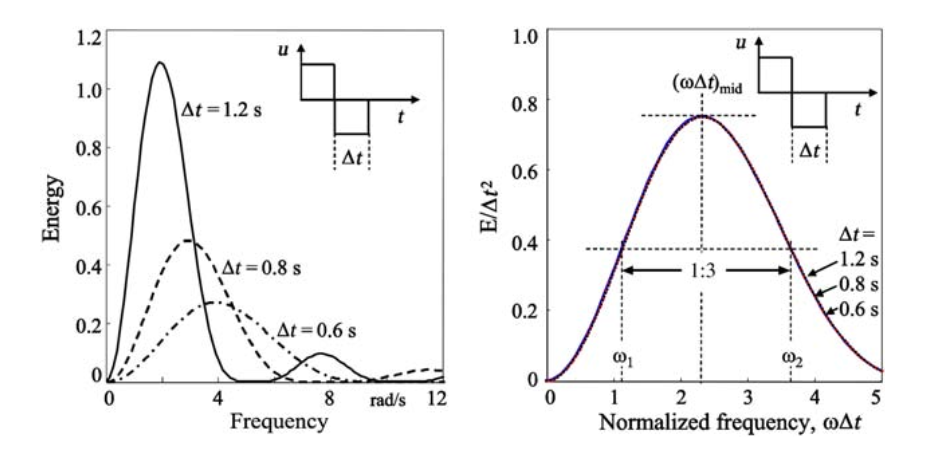
\includegraphics[width=0.8\textwidth]{Cap3/doblet.png}
    \caption{Doublet e seu espectro de energia para diferentes períodos $\Delta t$ \cite{Jategaonkar2015}.}
    \label{doublet}
\end{figure}

Portanto, a manobra adotada neste trabalho é o \textbf{doublet}, onde o comando é deslocado abruptamente em um sentido, mantido por um intervalo $\Delta t$, deslocado por igual intervalo no sentido oposto e, então, retornado à posição neutra. 
\begin{itemize}
    \item doublet no eixo de rolagem (excita a dinâmica de $p$),
    \item doublet no eixo de arfagem (excita $q$),
    \item doublet no eixo de guinada (excita $r$).
\end{itemize}

Trata-se de um sinal simétrico, cuja energia se concentra em torno de uma frequência que varia com $\Delta t$, conforme ilustra a Figura \ref{doublet}, o pico ocorre na frequência normalizada $\omega_n \Delta t \approx 2{,}3$, o que permite dimensionar a manobra a partir da frequência característica $\omega_n$ do canal a identificar \cite{Jategaonkar2015}:

\begin{equation}
\Delta t_{db} \approx \frac{2{,}3}{\omega_n} \approx \frac{T}{2{,}7},
\label{eq:doublet-dt}
\end{equation}

Na prática, adota-se a regra simplificada $2\Delta t_{db} \approx T$. Em torno do pico, o doublet apresenta largura de banda de aproximadamente $1{:}3$, faixa adequada para a estimação das derivadas de estabilidade e controle.

Em malha fechada, essas propriedades tornam-se ainda mais desejáveis. As reversões abruptas do doublet injetam energia rapidamente e exploram a resposta inicial da planta, antes de a realimentação reagir, mecanismo que \textcite{Jategaonkar2015} aponta como o que carrega a informação em malha fechada, enquanto a simetria e a curta duração mantêm as excursões pequenas, evitando a saturação do controlador.

Por fim, deve-se analisar a relação ruído-sinal, e o isolamento do sinal de cada eixo. Para isso é feita uma avaliação de cada janela de entrada, verificando-se o ruído de medição de cada eixo dos sensores, o qual é estimado de forma robusta a partir do resíduo de alta frequência do sinal, sendo esta a diferença entre a taxa medida $\omega_i$ e sua versão suavizada por um filtro Savitzky--Golay:
\begin{equation}
    \qquad e_i = \omega_i - \mathrm{SG}(\omega_i),
    \label{eq:ruido2}
\end{equation}
em que $\omega_i \in \{p,q,r\}$ é a taxa angular medida e o fator $1{,}4826$ converte o \textit{MAD} em um estimador do desvio-padrão de um ruído gaussiano $\sigma_{\eta,i}$, insensível aos transitórios da manobra. 
\begin{equation}
    \sigma_{\eta,i} = 1{,}4826 \cdot \operatorname{med}\big|\, e_i - \operatorname{med}(e_i) \,\big|
    \label{eq:ruido1}
\end{equation}

Isto permite calcular a relação sinal-ruído $\mathrm{SNR}_i$ de cada eixo que é, então, a razão entre o desvio-padrão da resposta na janela e esse ruído,
\begin{equation}
\mathrm{SNR}_i = \frac{\sigma(\omega_i)}{\sigma_{\eta,i}},
\label{eq:snr}
\end{equation}
e o isolamento $\rho_i$ mede o quanto a resposta se concentra no eixo-alvo em relação aos demais,
\begin{equation}
\rho_i = \frac{\sigma(\omega_i)}{\sqrt{\sum_{j \neq i} \sigma(\omega_j)^2}},
\label{eq:isolamento}
\end{equation}

A Tabela~\ref{tab:criterios} sintetiza os três critérios quantitativos.

\begin{table}[ht]
\centering
\caption{Critérios objetivos que caracterizam uma boa manobra de identificação.}
\label{tab:criterios}
\small
\begin{tabular}{@{}l c c p{3.7cm}@{}}
\toprule
Critério & Definição & Condição-alvo & Finalidade \\
\midrule
Largura do pulso, $\Delta t$ & $\dfrac{2{,}3}{\omega_n} \approx \dfrac{T}{2{,}7}$ \,(Eq.~\ref{eq:doublet-dt}) & $\omega_n\Delta t \approx 2{,}3$ & alocar a energia na banda do canal e $\approx 0$ em frequência nula \\[6pt]
Relação sinal--ruído, $\mathrm{SNR}_i$ & $\dfrac{\sigma(\omega_i)}{\sigma_{\eta,i}}$ \,(Eq.~\ref{eq:snr}) & $\mathrm{SNR}_i \geq 3$ & a resposta domina o ruído de medição \\[6pt]
Isolamento, $\rho_i$ & $\dfrac{\sigma(\omega_i)}{\sqrt{\sum_{j\neq i}\sigma(\omega_j)^2}}$ \,(Eq.~\ref{eq:isolamento}) & $\rho_i \gg 1$ & concentra a excitação no eixo-alvo \\
\bottomrule
\end{tabular}
\end{table}

Em síntese, a teoria define critérios objetivos que uma boa manobra deve satisfazer:
\begin{itemize}
    \item \textbf{Conteúdo de frequência:} energia concentrada na banda do canal-alvo ($\omega_n \Delta t \approx 2{,}3$) e praticamente nula em frequência zero;
    \item \textbf{Relação sinal--ruído:} razão $\geq 3$ entre a resposta devida à entrada e a devida ao ruído \cite{Jategaonkar2015};
    \item \textbf{Isolamento entre eixos:} excitação concentrada no eixo-alvo, com os demais quase inertes;
    \item \textbf{Faixa linear:} excursões pequenas, preservando a validade do modelo linearizado, sem saturar atuadores;
    \item \textbf{Retorno ao trim:} a simetria do doublet devolve a aeronave ao hover;
    \item \textbf{Repetibilidade:} manobra reproduzível de forma consistente entre ensaios.
\end{itemize}


\subsection{Aquisição de dados de saída (Measurements)}

A segunda etapa do M4V trata da obtenção e do condicionamento dos sinais medidos em voo. Seu objetivo é converter o dado bruto registrado pelos sensores em sinais limpos, uniformemente amostrados e livres de erros sistemáticos, e verificar a compatibilidade cinemática entre as grandezas medidas, garantindo que sejam mutuamente consistentes antes de alimentar o estimador. A exatidão das estimativas depende diretamente da qualidade dessas medidas, de modo que esta etapa é tão determinante quanto a escolha da manobra \cite{Jategaonkar2015, Tischler2012}. A Figura~\ref{fig:pipeline-dados} resume a cadeia de processamento, do log bruto ao vetor de medidas $z$.

\begin{figure}[ht]
    \centering
    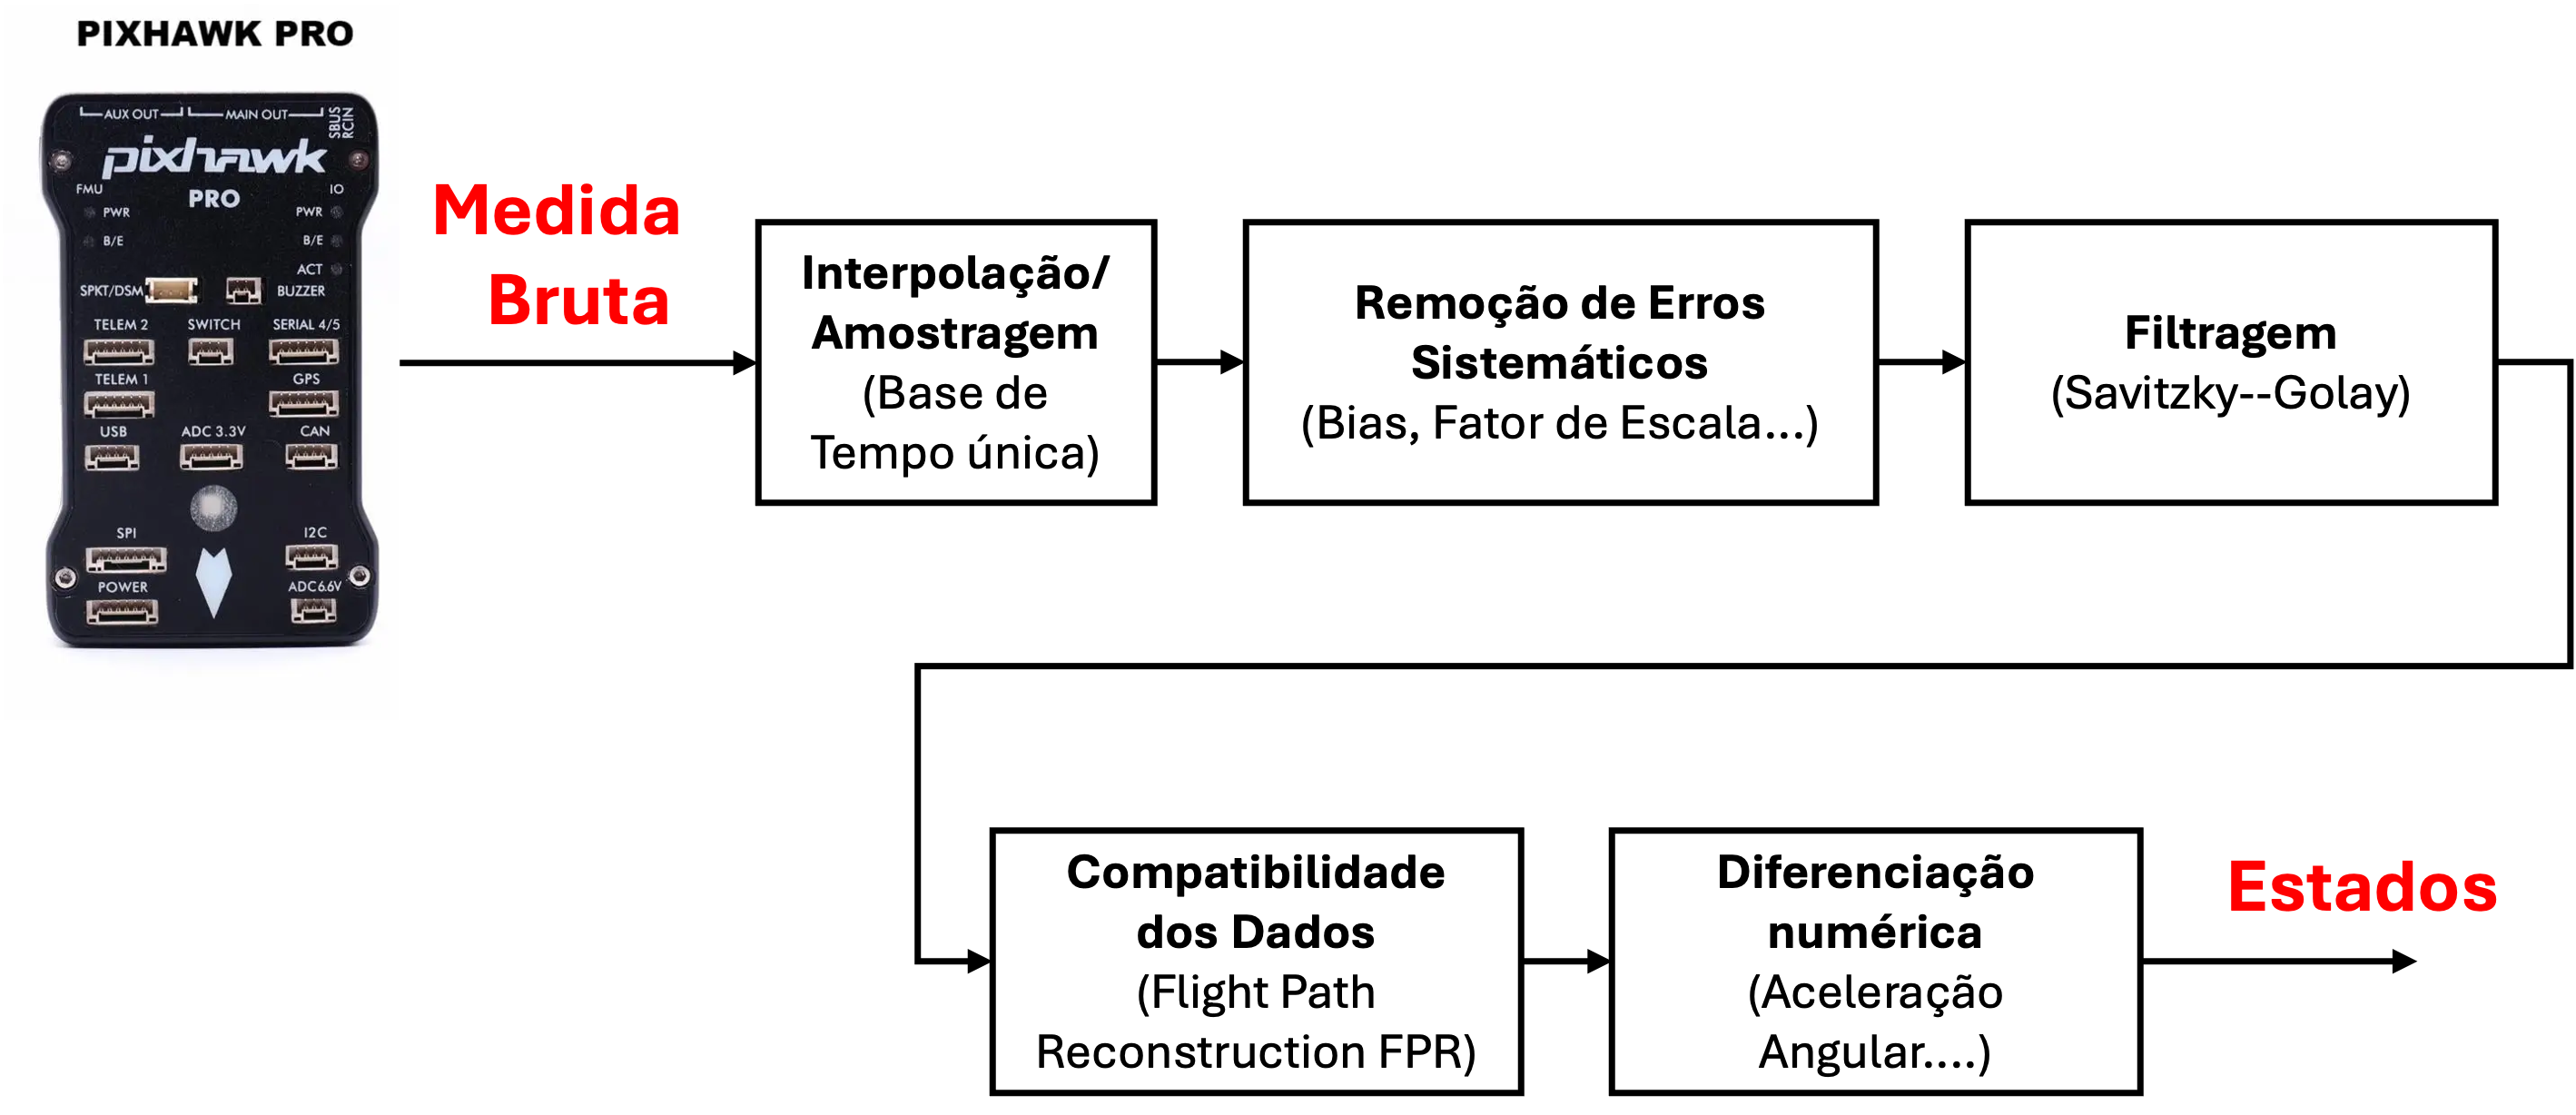
\includegraphics[width=0.95\textwidth]{Cap3/measure.png}
    \caption{Cadeia de aquisição e tratamento dos dados de voo.}
    \label{fig:pipeline-dados}
\end{figure}

Diferentemente da identificação de aeronaves de asa fixa, que requer deflexões de superfícies, ângulos de fluxo (incidência e derrapagem), pressão estática e demais dados de ar \cite{Jategaonkar2015, Sato2021}, o quadrirrotor em voo pairado dispensa a instrumentação de dados de ar: o modelo de corpo rígido do Capítulo~2 despreza a aerodinâmica translacional e os esforços provêm exclusivamente dos rotores. O conjunto de medidas reduz-se, então, às grandezas inerciais, à atitude e aos comandos, todas obtidas da controladora de voo (Pixhawk) e reunidas na Tabela~\ref{tab:medidas}. Cabe notar que a atitude $(\phi,\theta,\psi)$ não é medida diretamente, mas estimada pelo filtro de fusão (EKF) da controladora, combinando giroscópio, acelerômetro e magnetômetro; sua qualidade é aferida na verificação de compatibilidade descrita ao final desta seção.

\begin{table}[ht]
\centering
\caption{Grandezas medidas em voo e seu papel na identificação.}
\label{tab:medidas}
\small
\begin{tabular}{@{}l c l p{4.6cm}@{}}
\toprule
Grandeza & Símbolo & Fonte (sensor) & Papel na identificação \\
\midrule
Velocidades angulares & $p,q,r$ & giroscópio (IMU) & saída da dinâmica de taxa \\
Acelerações lineares & $a_x,a_y,a_z$ & acelerômetro (IMU) & saída (modelo do acelerômetro) \\
Atitude & $\phi,\theta,\psi$ & EKF da controladora & projeção da gravidade e compatibilidade \\
PWM dos motores & $\sigma_{1\text{--}4}$ & RCOU & entrada efetiva $u$ (via alocação) \\
Comando do piloto & $\boldsymbol{\sigma_P}$ & RCIN & entrada exógena (avaliação da manobra) \\
\bottomrule
\end{tabular}
\end{table}

Inicialmente trata-se a diferença entre as taxas de amostragem e tempos das amostras de todos os sensores. Pelo critério de Nyquist, a taxa de aquisição deve ser de, no mínimo, o dobro da maior frequência de interesse \cite{Jategaonkar2015}. Como a dinâmica de taxa do quadrirrotor concentra-se abaixo de aproximadamente $2$~Hz, adotou-se uma grade comum de $10$~Hz ($\Delta t = 0{,}1$~s), cerca de cinco vezes a banda do canal, mesma ordem de grandeza empregada por \textcite{Sato2021}, que utilizou $10$~Hz. Embora referências para aeronaves tripuladas recomendem $20$--$25$~Hz \cite{Jategaonkar2015}, para a banda de interesse deste trabalho $10$~Hz é suficiente para representar a dinâmica sem perda de informação.

Mesmo com sensores calibrados, persistem erros sistemáticos bias (deslocamento de zero) e fator de escala\cite{Jategaonkar2015, Sato2021}. O \textit{bias} dos sensores inerciais é estimado em janelas calmas (aeronave em repouso no solo ou em voo pairado estável): o do giroscópio é a mediana das taxas medidas (corpo sem rotação), e o do acelerômetro é a diferença entre a leitura mediana e a gravidade projetada no referencial do corpo pela atitude do EKF \cite{Jategaonkar2015}.

Para suprimir o ruído de alta frequência, não correlacionado com a dinâmica de interesse, aplica-se um filtro digital de Savitzky--Golay, o mesmo já empregado na avaliação das manobras na Equação~\eqref{eq:ruido2}. Por ser simétrico, esse filtro não introduz atraso de fase \cite{Jategaonkar2015}. O ponto essencial é que o \emph{mesmo} filtro é aplicado tanto à entrada (PWM) quanto à saída ($p,q,r,a$): como um filtro linear comuta com um sistema linear, esse procedimento preserva a relação entrada--saída e não cria defasagem relativa entre os sinais \cite{Tischler2012}.

O filtro de Savitzky--Golay ajusta, a cada instante $t_k$, um polinômio de grau $n$ a uma janela simétrica de $N = 2M+1$ amostras vizinhas por mínimos quadrados, substituindo a amostra central pelo valor ajustado. Reunindo a janela em $\mathbf{x}_k = [\,x_{k-M},\dots,x_{k+M}\,]^\top$ e o polinômio $p(i) = \sum_{j=0}^{n} a_j\,i^{\,j}$, com o índice $i$ contado a partir do centro da janela, os coeficientes resultam de
\begin{equation}
\hat{\mathbf{a}} = \arg\min_{\mathbf{a}} \sum_{i=-M}^{M}\!\bigg[\,x_{k+i} - \sum_{j=0}^{n} a_j\,i^{\,j}\,\bigg]^2 = \big(A^\top A\big)^{-1} A^\top \mathbf{x}_k,
\label{eq:sg-fit}
\end{equation}
em que $A \in \mathbb{R}^{N\times(n+1)}$, de elementos $A_{i,j} = i^{\,j}$, é a matriz de Vandermonde dos índices da janela. O valor suavizado é o polinômio avaliado no centro, $\tilde{x}_k = p(0) = \hat{a}_0$, o que equivale a uma convolução de coeficientes fixos,
\begin{equation}
\tilde{x}_k = \sum_{i=-M}^{M} h_i\, x_{k+i},
\qquad
\mathbf{h}^\top = \mathbf{e}_1^\top \big(A^\top A\big)^{-1} A^\top,
\label{eq:sg-conv}
\end{equation}
sendo $\mathbf{e}_1 = [\,1,0,\dots,0\,]^\top$ o vetor que extrai o coeficiente $\hat{a}_0$. Como $A$ depende apenas de $n$ e de $M$, os pesos $h_i$ são constantes e simétricos ($h_i = h_{-i}$), o que confirma a ausência de atraso de fase. Neste trabalho adotou-se ordem $n = 2$ e janela de $N = 7$ amostras ($M = 3$).

A aceleração angular não é medida diretamente, sendo obtida por diferenciação numérica das taxas já filtradas \cite{Jategaonkar2015}. Sua inclusão melhora a exatidão e a convergência da estimação e é necessária porque a aceleração angular entra diretamente no modelo do acelerômetro, Equação~\eqref{eq:acc-imu}, por meio do braço de alavanca da IMU. 

A Figura~\ref{fig:medidas-bias} ilustra o efeito da filtragem e da diferenciação no domínio do tempo, bem como a correção do bias, em um trecho do log de voo em que o drone está parado, e a Figura~\ref{fig:medidas-espectro}, apresenta a processamento dos dados medidos no intervalo de 605 s à 625 s.

\begin{figure}[ht]
    \centering
    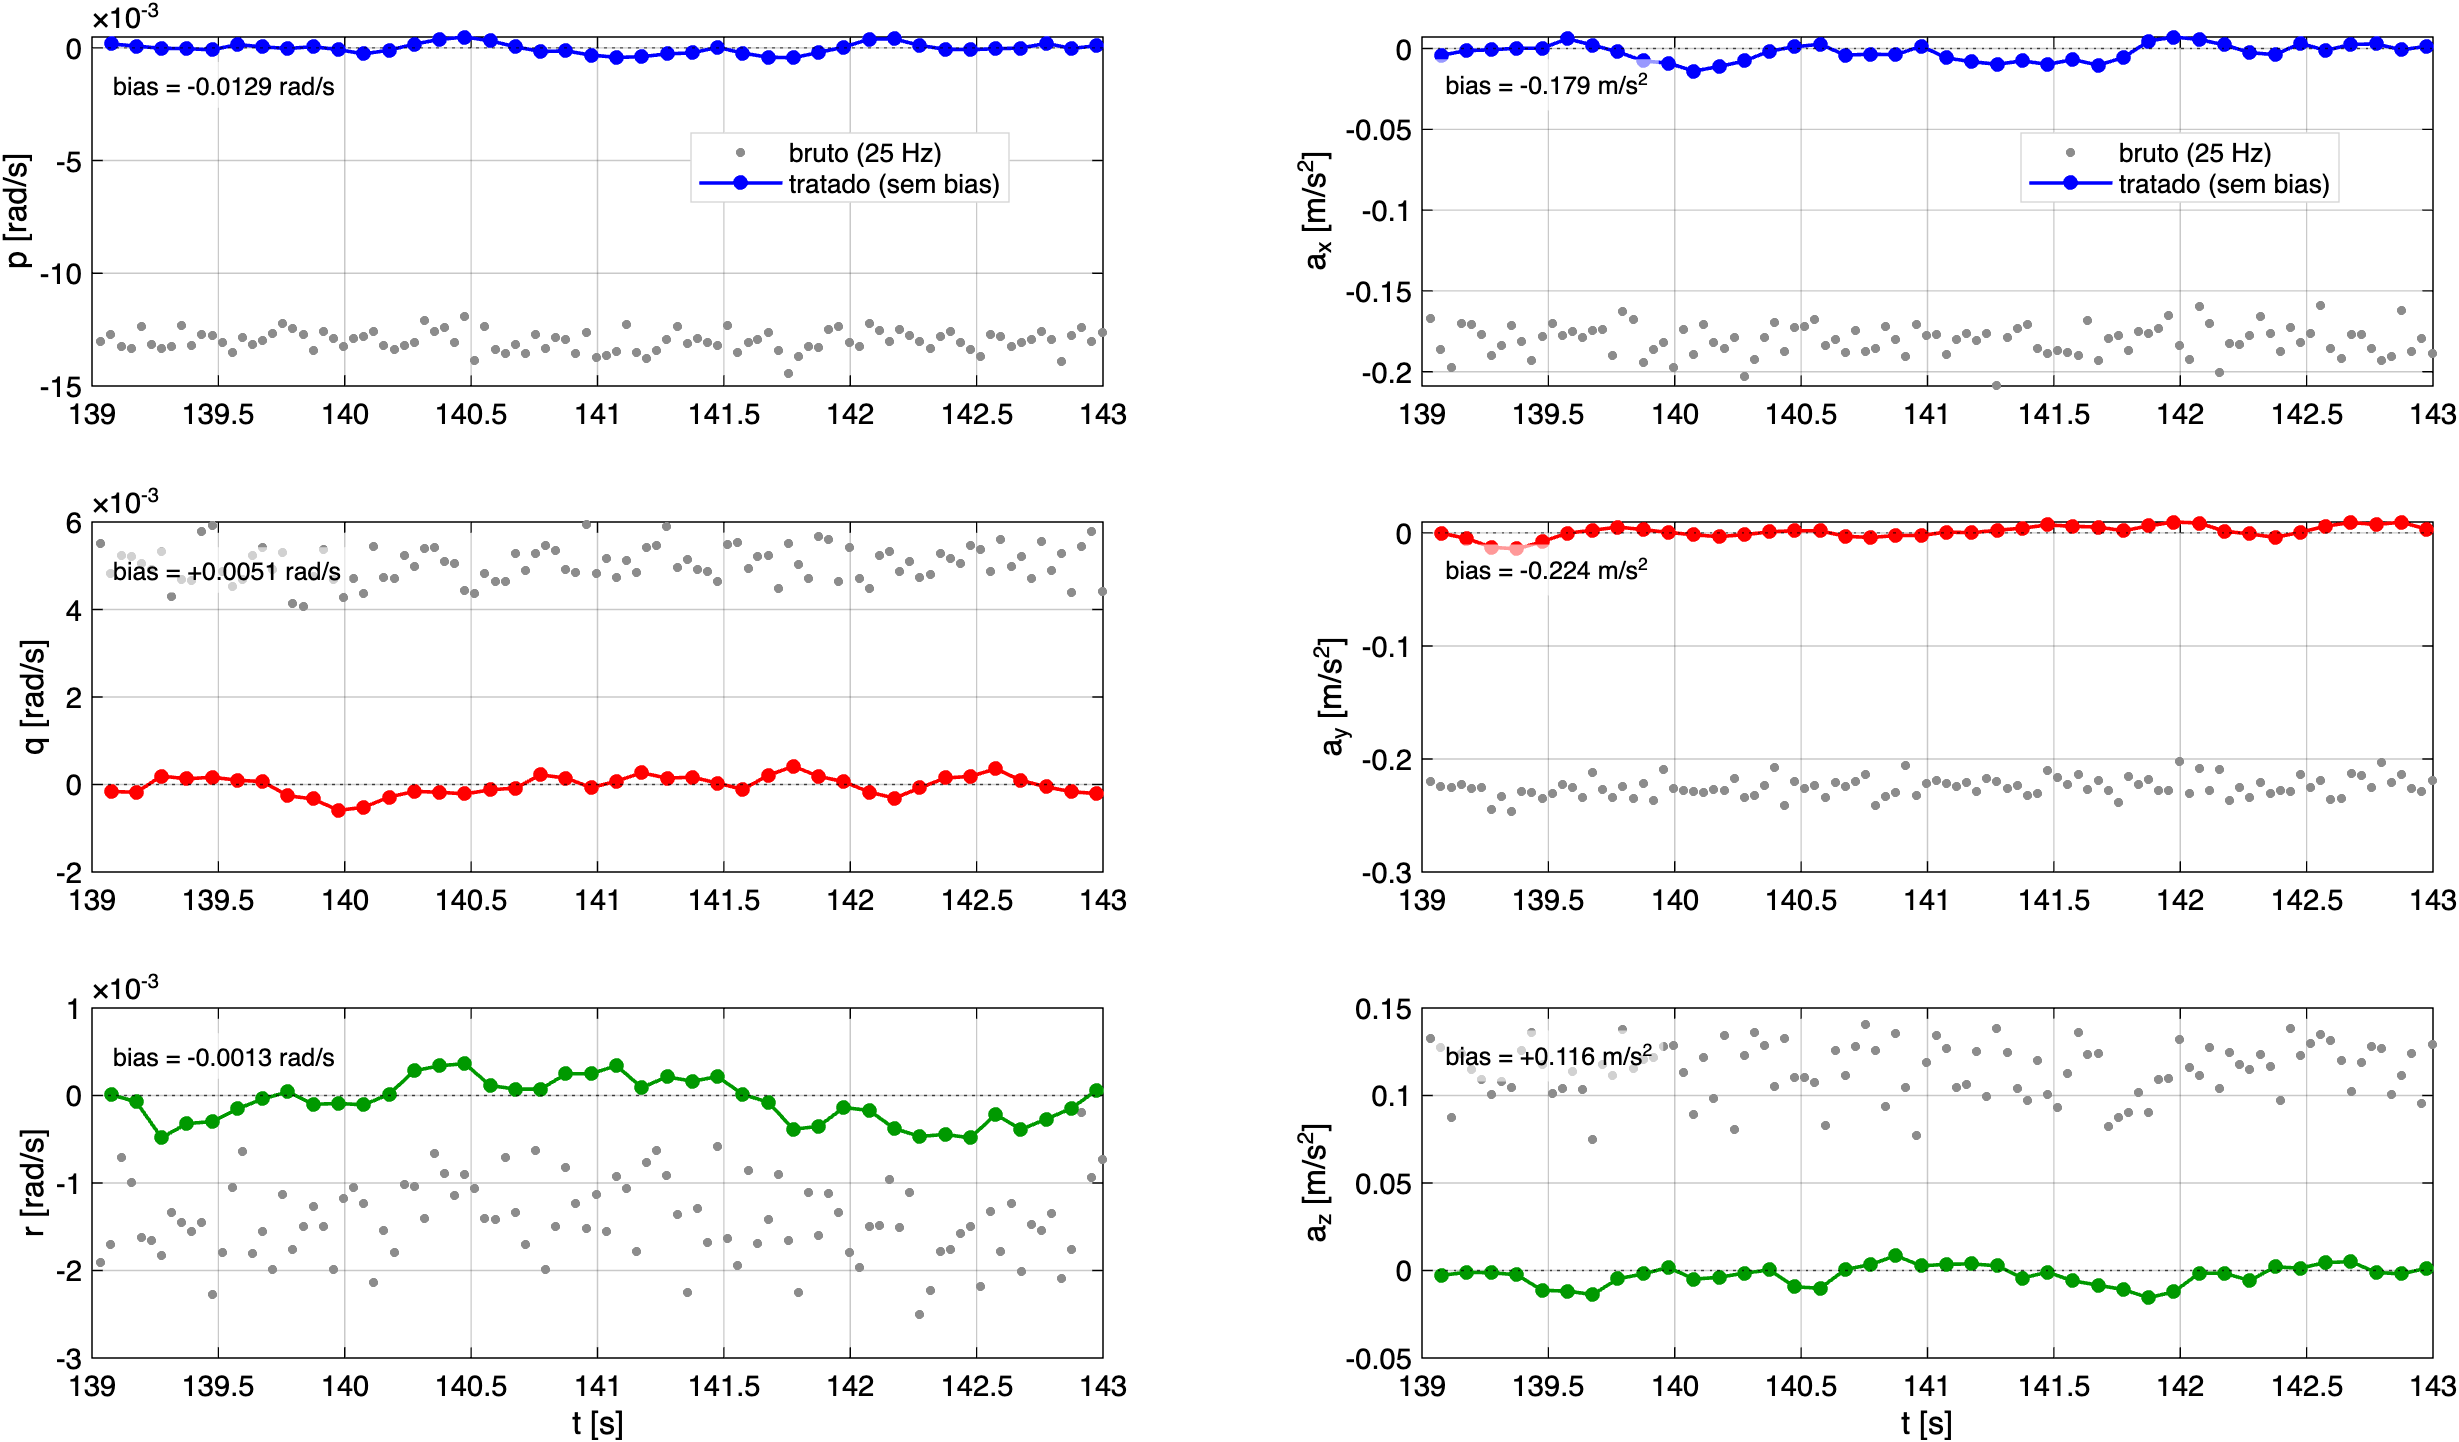
\includegraphics[width=0.9\textwidth]{Cap3/medidas_bias.png}
    \caption{Tratamento das medidas: calibração para correção de bias.}
    \label{fig:medidas-bias}
\end{figure}

\begin{figure}[ht]
    \centering
    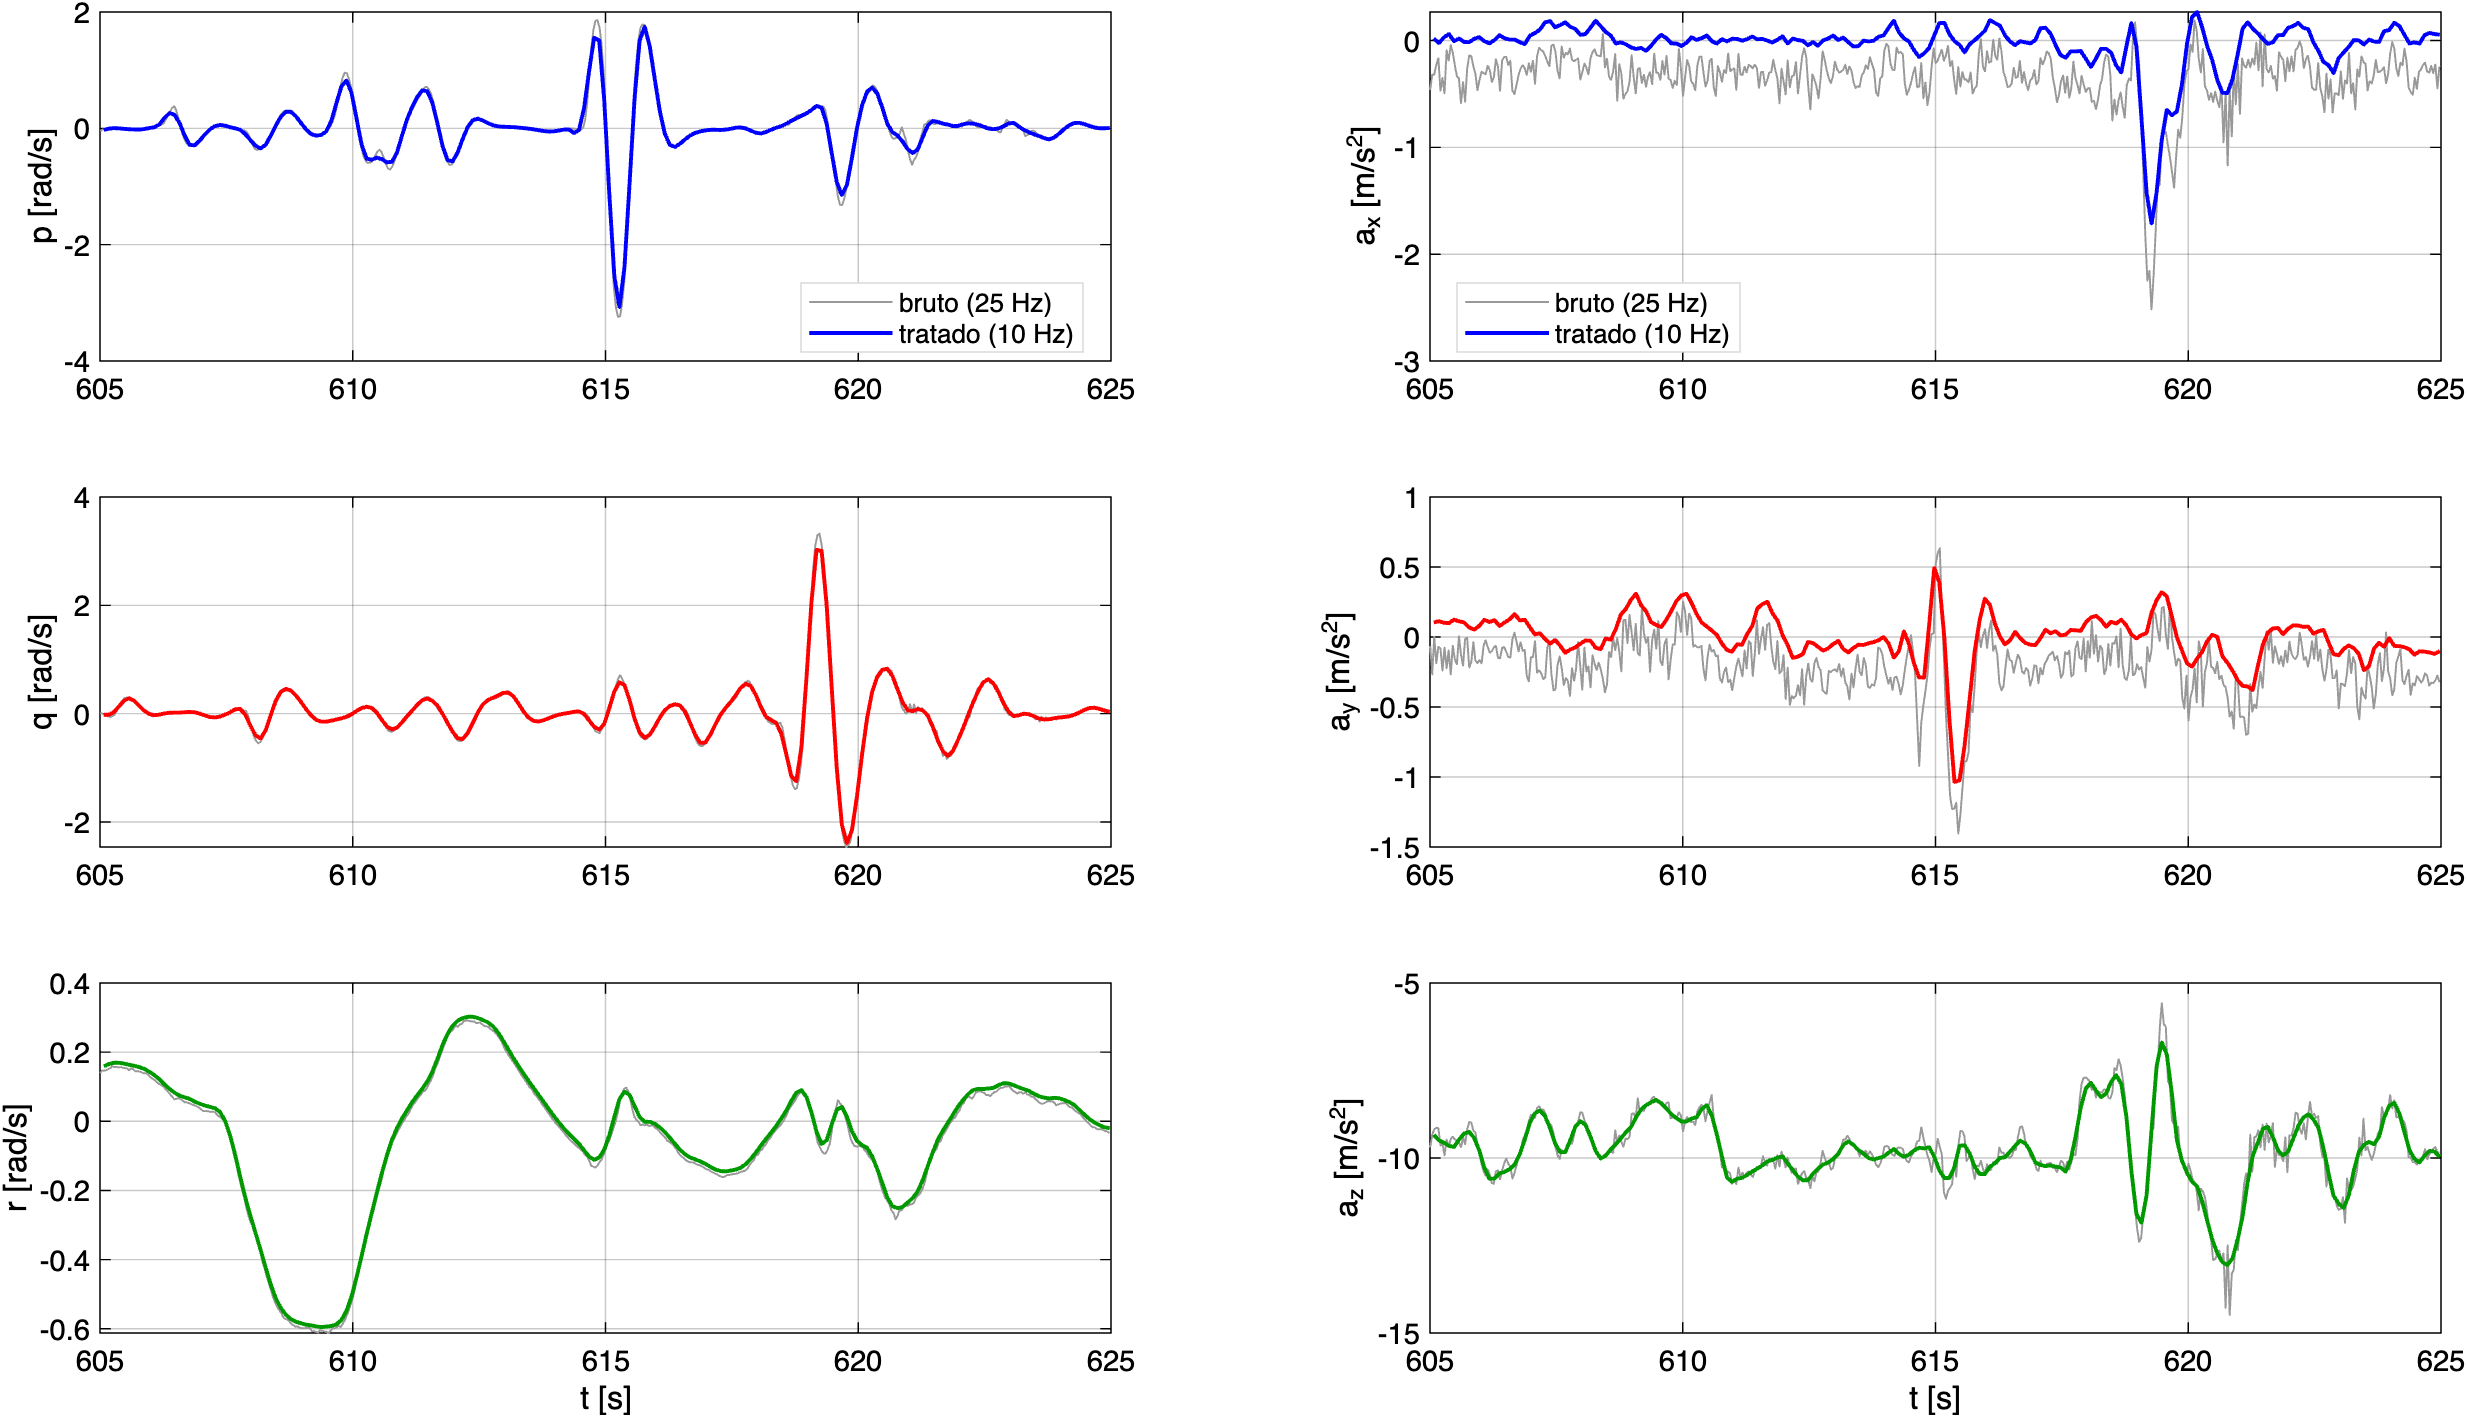
\includegraphics[width=0.9\textwidth]{Cap3/medidas_tratamento.png}
    \caption{Tratamento das medidas: efeito do processamento das medidas em intervalo de voo.}
    \label{fig:medidas-espectro}
\end{figure}

Ao final desta etapa, obtém-se o vetor de medidas $z$, velocidades angulares do giroscópio, forças específicas do acelerômetro e atitudes provenientes do EKF da pixhawk, em uma base de tempo uniforme, com erros sistemáticos removidos e consistência cinemática verificada, pronto para o método de identificação descrito a seguir.

\subsection{Identificação com dados pelo método OEM (Methods)}

A estimação dos parâmetros combina dois métodos complementares no domínio do tempo: o \textit{Equation Error Method} (EEM), a partir de um conjunto de parâmetros iniciais, $\Theta_{\text{0}}$, fornece uma estimativa algébrica dos parâmetros $\Theta_{\text{EEM}}$, e o \textit{Output Error Method} (OEM), que a refina por máxima verossimilhança até otimizar os parâmetros para $\Theta_{\text{OEM}}$ \cite{Jategaonkar2015}. Ambos buscam o vetor de parâmetros $\Theta$ que minimiza os resíduos entre a saída medida $z$ e a saída do modelo $y(\Theta)$.

O modelo de corpo rígido deduzido no Capítulo~2 descreve a dinâmica na forma de espaço de estados $\dot{\mathbf{x}} = f(\mathbf{x}, \mathbf{u}, \Theta)$, com o estado completo: 

$\mathbf{x} = [\,p,q,r,\phi,\theta,\psi,u,v,w\,]^\top$ 
e a entrada,

$\mathbf{u} = [\,T,\tau_x,\tau_y,\tau_z\,]^\top$ (empuxo total e momentos de controle reconstruídos dos comandos PWM). O vetor de parâmetros a identificar é
\begin{equation}
    \Theta = [\,J_x,\,J_y,\,J_z,\,J_{xz},\;{c_T}_1,\dots,{c_T}_4,\;{c_M}_1,\dots,{c_M}_4,\;c_p,\,c_q,\,c_r\,]^\top,
    \label{eq:theta}
\end{equation}
reunindo os momentos de inércia, os coeficientes de empuxo ${c_T}_i$ e de contra-torque ${c_M}_i$ de cada motor (Equações~\eqref{eq:motor-thrust} e~\eqref{eq:motor-torque}, refinados por motor a partir dos ensaios de bancada do Apêndice~\ref{ap:bancada}).

\begin{table}[ht]
    \centering
    \caption{Nomenclatura dos parâmetros $\Theta$ e a origem de cada parâmetro.}
    \label{tab:p0}
    \footnotesize
    \setlength{\tabcolsep}{5pt}
    \begin{tabular}{l c c l}
    \toprule
    Nome & Parâmetro & Dimensão & Origem \\
    \midrule
    Momento de inércia em rolagem           & $J_x$     & kg$\cdot$m$^2$    & CAD \\
    Momento de inércia em arfagem           & $J_y$     & kg$\cdot$m$^2$    & CAD \\
    Momento de inércia em guinada           & $J_z$     & kg$\cdot$m$^2$    & CAD \\
    Produto de inércia                      & $J_{xz}$  & kg$\cdot$m$^2$    & CAD \\
    Coeficiente de empuxo do motor 1        & ${c_T}_1$ & N/RPM$^2$         & bancada (Apêndice~\ref{ap:bancada}) \\
    Coeficiente de empuxo do motor 2        & ${c_T}_2$ & N/RPM$^2$         & bancada (Apêndice~\ref{ap:bancada}) \\
    Coeficiente de empuxo do motor 3        & ${c_T}_3$ & N/RPM$^2$         & bancada (Apêndice~\ref{ap:bancada}) \\
    Coeficiente de empuxo do motor 4        & ${c_T}_4$ & N/RPM$^2$         & bancada (Apêndice~\ref{ap:bancada}) \\
    Coeficiente de contra-torque do motor 1 & ${c_M}_1$ & N$\cdot$m/RPM$^2$ & bancada (Apêndice~\ref{ap:bancada}) \\
    Coeficiente de contra-torque do motor 2 & ${c_M}_2$ & N$\cdot$m/RPM$^2$ & bancada (Apêndice~\ref{ap:bancada}) \\
    Coeficiente de contra-torque do motor 3 & ${c_M}_3$ & N$\cdot$m/RPM$^2$ & bancada (Apêndice~\ref{ap:bancada}) \\
    Coeficiente de contra-torque do motor 4 & ${c_M}_4$ & N$\cdot$m/RPM$^2$ & bancada (Apêndice~\ref{ap:bancada}) \\
    Coeficiente de amortecimento em rolagem & $c_p$     & s$^{-1}$          & estimativa inicial empírica \\
    Coeficiente de amortecimento em arfagem & $c_q$     & s$^{-1}$          & estimativa inicial empírica \\
    Coeficiente de amortecimento em guinada & $c_r$     & s$^{-1}$          & estimativa inicial empírica \\
    \bottomrule
    \end{tabular}
\end{table}

A identificação concentra-se no subsistema rotacional. Como as Equações~\eqref{eq:p_dot}--\eqref{eq:r_dot} são autônomas nas velocidades angulares, suas derivadas dependem apenas de $(p,q,r)$ e dos momentos $\tau_x,\tau_y,\tau_z$, basta integrar esse subsistema, comparando as taxas simuladas e as forças específicas do acelerômetro (Equações~\eqref{eq:acc-x}--\eqref{eq:acc-z}) às medições.

A metodologia utilizada une dois métodos de identificação para alcançar um modelo final, \gls{EEM} e \gls{OEM}, com auxílio de um técnica para utilização de multijanelas progressivas. Figura~\ref{fig:oem-pipeline} resume esse processo:

\begin{figure}[ht]
    \centering
    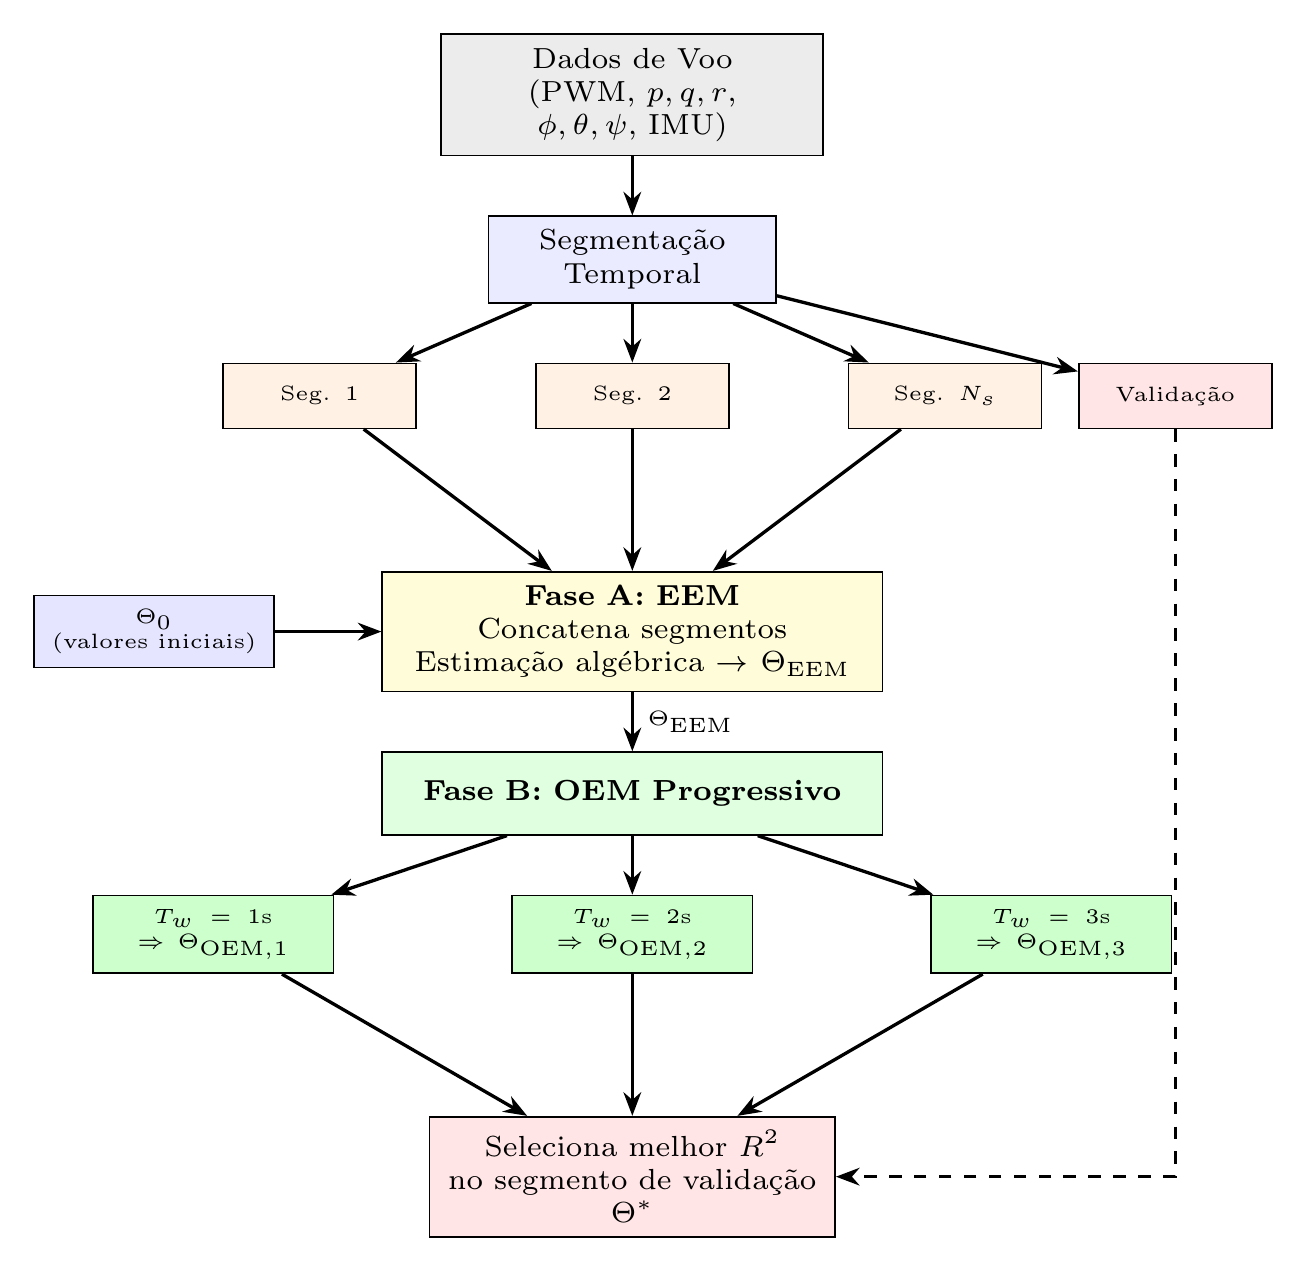
\includegraphics[width=0.9\textwidth]{Cap3/oem_pipeline.png}
    \caption{Processo de identificação em duas fases EEM + OEM.}
    \label{fig:oem-pipeline}
\end{figure}

\textbf{Fase A --- EEM (estimativa inicial).} O EEM dispensa a integração numérica: avalia a equação dinâmica diretamente sobre os estados medidos e suas derivadas. Definindo o resíduo de equação como a diferença entre a derivada angular medida e a prevista pelas Equações~\eqref{eq:p_dot}--\eqref{eq:r_dot},
\begin{equation}
e_{\text{EEM}}(t_k) = \dot{\boldsymbol{\omega}}_{\text{med}}(t_k) - f_\omega\big(\boldsymbol{\omega}_{\text{med}}(t_k),\, \boldsymbol{\tau}(t_k),\, \Theta\big),
\label{eq:eem-res}
\end{equation}
com $\boldsymbol{\omega} = [p,q,r]^\top$, os parâmetros são obtidos minimizando o erro quadrático ponderado sobre os segmentos de treino concatenados,
\begin{equation}
\Theta_{\text{EEM}} = \arg\min_{\Theta} \sum_{k} \big\| W^{1/2}\, e_{\text{EEM}}(t_k) \big\|^2,
\label{eq:eem-cost}
\end{equation}
em que $W = \mathrm{diag}(1/\sigma_{y_i}^2)$ pondera cada eixo pelo inverso da variância de sua derivada, sendo $\sigma_{y_i}$ o desvio-padrão do canal de saída $i$ (a não confundir com o comando $\sigma_i$ do motor), e $\dot{\boldsymbol{\omega}}_{\text{med}}$ é obtida por diferenciação numérica do sinal suavizado. Com as inércias fixadas, a Equação~\eqref{eq:eem-res} é linear nos ganhos e nos coeficientes de arrasto, tornando \eqref{eq:eem-cost} um problema de mínimos quadrados de solução rápida e robusta. Em contrapartida, o uso das derivadas medidas --- que amplificam o ruído --- introduz viés, razão pela qual o EEM serve como ponto de partida, e não como estimativa final \cite{Jategaonkar2015}.

\textbf{Fase B --- OEM (refinamento).} O OEM elimina esse viés ao comparar a saída \emph{integrada} do modelo com a medição. A partir de $\Theta_{\text{EEM}}$, integra-se o subsistema de taxa no tempo (Runge--Kutta de 4ª ordem) com a mesma entrada aplicada ao veículo, produzindo $y(t_k,\Theta)$; o resíduo é o \emph{erro de saída} $z(t_k) - y(t_k,\Theta)$, conforme ilustra a Figura~\ref{fig:oem-loop}. As saídas $z,y$ reúnem as velocidades angulares $(p,q,r)$ e as forças específicas medidas pela IMU $(a_x,a_y,a_z)$, estas últimas sensíveis ao empuxo total $T$ e, por meio do braço do sensor, à aceleração angular.

Sob a hipótese de ruído de medição gaussiano com covariância $R$, o OEM é um estimador de máxima verossimilhança: minimiza o custo (log-verossimilhança negativa)
\begin{equation}
J(\Theta) = \tfrac{1}{2}\sum_{k=1}^{N} \big[z(t_k) - y(t_k,\Theta)\big]^\top R^{-1} \big[z(t_k) - y(t_k,\Theta)\big].
\label{eq:oem-cost}
\end{equation}
O mínimo é buscado pelo método de Gauss--Newton. Linearizando a saída em torno da estimativa corrente, $y(\Theta + \delta) \approx y(\Theta) + S\,\delta$, com a \emph{matriz de sensibilidades}
\begin{equation}
S(t_k) = \frac{\partial y(t_k,\Theta)}{\partial \Theta},
\label{eq:sens}
\end{equation}
o passo $\delta$ que anula o gradiente do custo resolve as equações normais
\begin{equation}
\underbrace{\Bigg[\textstyle\sum_{k} S_k^\top R^{-1} S_k\Bigg]}_{\textstyle F\ \text{(informação de Fisher)}} \delta \;=\; \sum_{k} S_k^\top R^{-1}\big[z(t_k) - y(t_k,\Theta)\big],
\label{eq:gauss-newton}
\end{equation}
e os parâmetros são atualizados por
\begin{equation}
\Theta_{j+1} = \Theta_j + \delta,
\label{eq:update}
\end{equation}
repetindo-se o ciclo de integrar o modelo, formar o erro de saída, calcular as sensibilidades e atualizar, até a convergência (Figura~\ref{fig:oem-loop}). Neste trabalho, as sensibilidades $S$ são calculadas por diferenças finitas, a covariância $R$ é aproximada pela matriz diagonal fixa $W = \mathrm{diag}(1/\sigma_{y_i}^2)$, e o passo $\delta$ é determinado pelo algoritmo \textit{trust-region reflective} da função \texttt{lsqnonlin}, que globaliza o Gauss--Newton e impõe os limites físicos dos parâmetros, resultando em um $\Theta_{\text{OEM}}$.

\begin{figure}[ht]
    \centering
    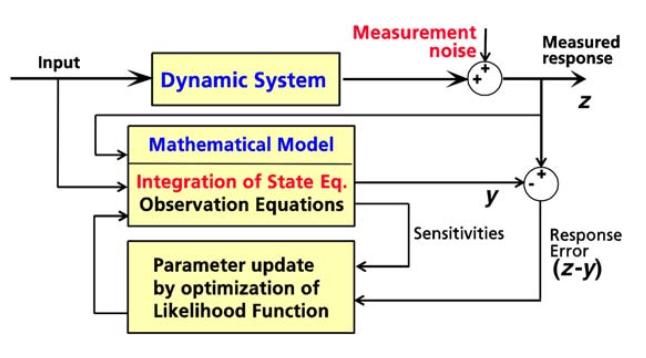
\includegraphics[width=0.65\textwidth]{Cap3/oem_loop.png}
    \caption{Ciclo iterativo do método do erro de saída \cite{Jategaonkar2015}.}
    \label{fig:oem-loop}
\end{figure}

\textbf{Estratégia de multijanelas progressivas.} A integração de um sistema instável em malha aberta pode divergir. Para conter isso, cada segmento de treino é dividido em janelas curtas; no início de cada janela o estado do modelo é reinicializado com o valor medido, impedindo que erros de integração se propaguem entre janelas. A duração das janelas cresce progressivamente, $T_w = 1\,\text{s} \to 2\,\text{s} \to 3\,\text{s}$: as etapas curtas ajustam os parâmetros com baixo risco de divergência e as longas capturam a dinâmica de mais longo prazo. O custo do OEM agrega os resíduos de todas as janelas de todos os segmentos de treino, mas para reduzir o erro acumulado entre o modelo simulado e o medido, a cada final de janela o valor do modelo é atualizado para o valor da medida.
\begin{equation}
J(\Theta) = \sum_{s=1}^{N_s} \sum_{w} \sum_{k \in \mathcal{W}_w^{(s)}} \big\| W^{1/2}\big[z(t_k) - y(t_k,\Theta)\big]\big\|^2,
\label{eq:oem-multiwin}
\end{equation}
em que $N_s$ é o número de segmentos e $\mathcal{W}_w^{(s)}$ os índices da janela $w$ do segmento $s$. Ao fim de cada estágio o modelo é avaliado no segmento de validação, que não participa da otimização, pelo coeficiente de determinação
\begin{equation}
R^2 = 1 - \frac{\sum_k (z_k - y_k)^2}{\sum_k (z_k - \bar{z})^2},
\label{eq:r2}
\end{equation}
e o conjunto de parâmetros com maior $R^2$ médio é tomado como resultado final $\Theta_{\text{OEM}}$.

Na convergência, a inversa da matriz de informação de Fisher fornece a covariância das estimativas, $\mathrm{Cov}(\Theta) \approx \sigma^2 \big(S^\top W S\big)^{-1} = \sigma^2 F^{-1}$ (limite de Cramér--Rao), de onde se extrai o desvio-padrão relativo de cada parâmetro. Valores elevados sinalizam parâmetros pouco observáveis pelos dados.

\subsection{Modelo não linear para identificação (Models)}

A etapa de modelos define a estrutura matemática que liga as entradas às saídas medidas, cujos parâmetros físicos serão estimados. Adota-se uma abordagem de caixa cinza: a estrutura é fixada pelas leis de corpo rígido deduzidas no Capítulo~2 (cinemática e equações de Newton--Euler), enquanto apenas os parâmetros físicos são estimados a partir dos dados de voo \cite{Aguirre2015}. Como as equações cinemáticas são bem estabelecidas, a confiabilidade da identificação depende sobretudo da adequação do modelo postulado \cite{Jategaonkar2015}.

Seguindo \textcite{Jategaonkar2015}, o processo é escrito na forma geral de espaço de estados:
\begin{align}
\dot{\mathbf{x}}(t) &= f[\mathbf{x}(t),\mathbf{u}(t),\Theta], \quad \mathbf{x}(t_0)=\mathbf{x}_0, \label{eq:model-fx}\\
\mathbf{y}(t) &= g[\mathbf{x}(t),\mathbf{u}(t),\Theta], \label{eq:model-gy}\\
\mathbf{z}(t_k) &= \mathbf{y}(t_k) + \mathbf{v}(t_k), \label{eq:model-z}
\end{align}
em que $f$ é a função dinâmica (equações de movimento), $g$ a função de saída (modelo de sensor), $\mathbf{z}$ as medições amostradas nos instantes $t_k$, corrompidas pelo ruído $\mathbf{v}$, e $\Theta$ o vetor de parâmetros a identificar.

Embora o corpo rígido tenha nove estados, a identificação reduz-se ao subsistema rotacional, pois é nele que aparecem os parâmetros de interesse e porque as Equações~\eqref{eq:p_dot}--\eqref{eq:r_dot} são autônomas nas velocidades angulares. Toma-se, portanto,
\begin{equation}
\mathbf{x}=[\,p,q,r,\phi,\theta,\psi,u,v,w\,]^{\top}, \qquad \mathbf{u}=[\,T,\,\tau_x,\,\tau_y,\,\tau_z\,]^{\top}.
\label{eq:model-xu}
\end{equation}

As entradas não são medidas diretamente, mas são reconstruídas dos comandos PWM em duas etapas. Primeiro, o modelo de propulsão converte cada comando $\sigma_i$ em empuxo e contra-torque, ${T_i={c_T}_i\,\Omega_i^{2}}$ e ${Q_i={c_M}_i\,\Omega_i^{2}}$ (Equações~\eqref{eq:motor-thrust} e~\eqref{eq:motor-torque}); em seguida, a matriz de alocação~\eqref{eq:alocacao} combina-os no empuxo total e nos momentos $(T,\tau_x,\tau_y,\tau_z)$. Assim, a própria entrada depende de parâmetros de $\Theta$ (os ${c_T}_i$ e ${c_M}_i$), traço característico da formulação em caixa cinza.

A dinâmica de taxa é dada pelas Equações~\eqref{eq:p_dot}--\eqref{eq:r_dot}, em que os coeficientes $\Gamma_i$ são funções dos momentos de inércia $(J_x,J_y,J_z,J_{xz})$ e $c_p,c_q,c_r$ são os arrastos angulares. O modelo é não linear, portanto, os termos giroscópicos $pq$, $qr$ e $pr$ acoplam os três eixos, e a assimetria de inércia ($J_{xz}\neq 0$, herdada da fuselagem de asa fixa) acopla rolagem e guinada, afastando-o das formulações desacopladas usuais de multirrotores simétricos.

\begin{figure}[ht]
    \centering
    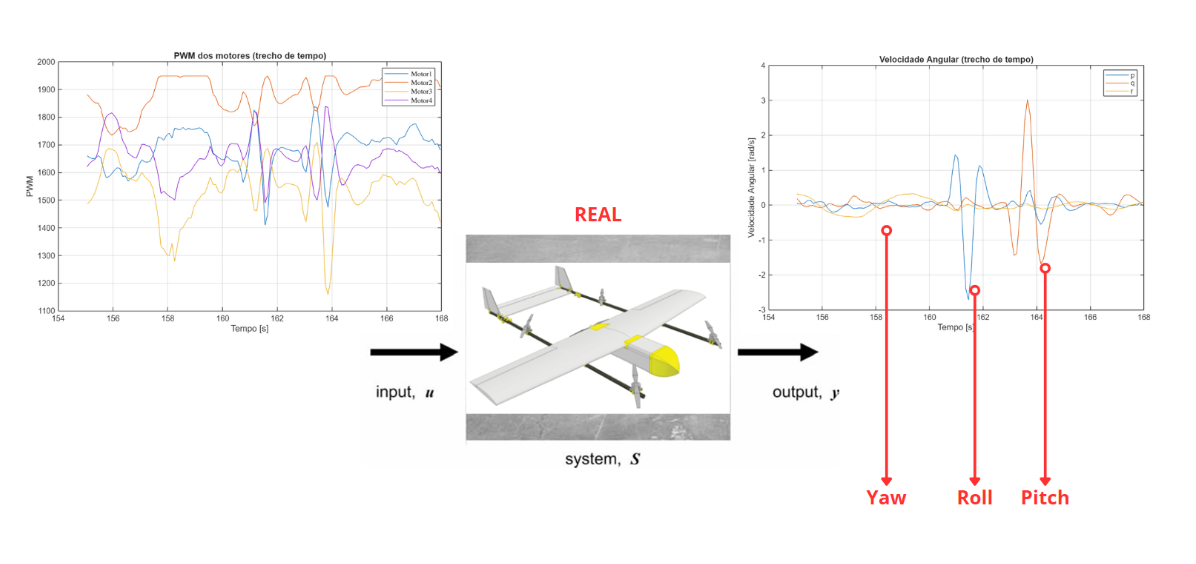
\includegraphics[width=0.9\textwidth]{Cap3/inout.png}
    \caption{Modelo relacionando entradas com as saídas medidas \cite{Jategaonkar2015}.}
    \label{fig:inout}
\end{figure}

As grandezas observadas reúnem as taxas angulares (giroscópio) e as forças específicas (acelerômetro):
\begin{equation}
\mathbf{y}=[\,p,\,q,\,r,\;a_x,\,a_y,\,a_z\,]^{\top}.
\label{eq:model-y}
\end{equation}

As taxas compõem $g$ diretamente as acelerações que seguem o modelo de sensor com braço de alavanca, Equações~\eqref{eq:acc-x}--\eqref{eq:acc-z}. Por esse acoplamento, o acelerômetro carrega informação sobre a aceleração angular $(\dot p,\dot q,\dot r)$ e sobre o empuxo $T/m$, o que é explorado na estimação dos coeficientes de inércia e de propulsão.

O vetor a identificar é o $\Theta$ da Equação~\eqref{eq:theta}, reunindo as inércias, os coeficientes ${c_T}_i$ e ${c_M}_i$ de cada rotor e os arrastos $c_p,c_q,c_r$. O modelo pressupõe corpo rígido em modo quadrirrotor, com velocidade longitudinal desprezível, eliminando sustentação e arrastos da estrutura de asa fixa, e, operação em torno do voo pairado, condição em que o subsistema rotacional fica fracamente acoplado à translação. Conforme a análise de identificabilidade recomendada por \textcite{Jategaonkar2015}, os parâmetros pouco observáveis.

\subsection{Critérios para validação no domínio do tempo (Validation)}

A última etapa compara o modelo identificado com um segmento de validação, o qual possue movimento composto não utilizado durante a estimação, comparando a saída simulada $y$ com a medida $z$ em cada canal ($p,q,r,a_x,a_y,a_z$). Empregam-se quatro métricas complementares: Coeficiente de determinação ($R^2$) e coeficiente de Theil(TIC), a Decomposição de Theil ($U^b, U^v, U^c$), e o Limite de Cramér-Rao.

\textbf{Coeficiente de determinação ($R^2$).} Definido na Equação~\eqref{eq:r2}, mede a fração da variância dos dados explicada pelo modelo; $R^2=1$ indica o modelo perfeito. A partir de 0.5 é considerado um modelo aceitável, porém, apesar de ter leitura imediata, penaliza fortemente erros de offset e de escala, distorcendo um pouco a análise.

\textbf{Coeficiente de inequação de Theil (TIC).} É uma medida normalizada do erro, limitada ao intervalo $[0,1]$,
\begin{equation}
\mathrm{TIC} = \frac{\sqrt{\tfrac{1}{N}\sum_k (z_k - y_k)^2}}{\sqrt{\tfrac{1}{N}\sum_k z_k^2} + \sqrt{\tfrac{1}{N}\sum_k y_k^2}},
\label{eq:tic}
\end{equation}
em que $\mathrm{TIC}=0$ corresponde ao ajuste perfeito e $\mathrm{TIC}=1$ é um modelo totalmente incorreto. Por ser adimensional e normalizada, permite comparar canais de magnitudes distintas; \textcite{Jategaonkar2015} considera $\mathrm{TIC} \lesssim 0{,}25$--$0{,}30$ indicativo de um bom modelo.

\textbf{Decomposição de Theil.} O erro quadrático médio, $\mathrm{MSE}=\tfrac{1}{N}\sum_k (z_k-y_k)^2$, separa-se em três parcelas que somam a unidade,
\begin{align}
U^{b} = \frac{(\bar{z}-\bar{y})^2}{\mathrm{MSE}}, \qquad
U^{v} = \frac{(\sigma_z-\sigma_y)^2}{\mathrm{MSE}}, \qquad
U^{c} = \frac{2(1-\rho)\,\sigma_z\,\sigma_y}{\mathrm{MSE}},
\label{eq:theil}
\end{align}
com $U^{b}+U^{v}+U^{c}=1$, sendo $\bar{z},\bar{y}$ as médias, $\sigma_z,\sigma_y$ os desvios-padrão e $\rho$ a correlação entre medida e simulação. 

A parcela de \emph{viés} $U^{b}$ capta erro sistemático de offset; a de \emph{variância} $U^{v}$, discrepância de amplitude (amortecimento ou ganho mal capturados); e a de \emph{covariância} $U^{c}$, o erro não sistemático (aleatório). O ideal é $U^{b}\approx 0$, $U^{v}\approx 0$ e $U^{c}\approx 1$: o resíduo concentra-se na parcela aleatória, sem componente estrutural --- indício de que a dinâmica foi corretamente capturada e o que resta é ruído \cite{Jategaonkar2015}.

\textbf{Limite de Cramér--Rao.} Diferentemente das anteriores, que avaliam o \emph{ajuste}, o limite de Cramér--Rao avalia a \emph{confiabilidade dos parâmetros}. Da inversa da matriz de informação de Fisher, introduzida na etapa de métodos, extrai-se o desvio-padrão relativo de cada parâmetro; seguindo \textcite{Tischler2012} e \textcite{Sato2021}, valores abaixo de $20\%$ caracterizam um parâmetro bem identificado, enquanto valores superiores apontam baixa observabilidade, tipicamente os parâmetros do canal de guinada.